%-------------------------------------------------------------------------------------------------------------------------------------------------------------------------------------------------
% Section 3
%
%-------------------------------------------------------------------------------------------------------------------------------------------------------------------------------------------------
\section{Properties of Bernoulli line ensembles}\label{Section3} In this section we derive several results for Bernoulli line ensembles, which will be used in the proof of Theorem \ref{PropTightGood} in Section \ref{Section4}.


%-------------------------------------------------------------------------------------------------------------------------------------------------------------------------------------------------
% Section 3.1
%
%-------------------------------------------------------------------------------------------------------------------------------------------------------------------------------------------------
\subsection{Monotone coupling lemmas}\label{Section3.1}
 In this section we formulate two lemmas that provide couplings of two Bernoulli line ensembles of non-intersecting Bernoulli bridges on the same interval, which depend monotonically on their boundary data. Schematic depictions of the couplings are provided in Figure \ref{fig:MCL}. We postpone the proof of these lemmas until Section \ref{AppendixA}. 
\begin{figure}[ht]
\begin{center}
  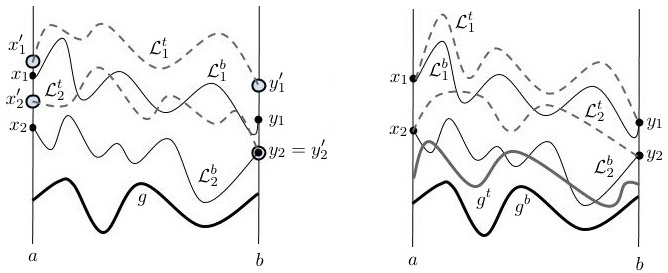
\includegraphics[scale = 0.8]{S2_1_new.jpg}
  \caption{Two diagrammatic depictions of the monotone coupling Lemma \ref{MCLxy} (left part) and Lemma \ref{MCLfg} (right part).}
  \label{fig:MCL}
  \end{center}
\end{figure}

\begin{lemma}\label{MCLxy} Assume the same notation as in Definition \ref{DefAvoidingLawBer}. Fix $k \in \mathbb{N}$, $T_0, T_1 \in \mathbb{Z}$ with $T_0 < T_1$, a function $g: \llbracket T_0, T_1 \rrbracket  \rightarrow [-\infty, \infty)$ as well as $\vec{x}, \vec{y}, \vec{x}\,', \vec{y}\,' \in \mathfrak{W}_k$. Assume that $\Omega_{avoid}(T_0, T_1, \vec{x}, \vec{y}, \infty,g)$ and $\Omega_{avoid}(T_0, T_1, \vec{x}', \vec{y}', \infty,g)$ are both non-empty. Then there exists a probability space $(\Omega, \mathcal{F}, \mathbb{P})$, which supports two $\llbracket 1, k \rrbracket$-indexed Bernoulli line ensembles $\mathfrak{L}^t$ and $\mathfrak{L}^b$ on $\llbracket T_0, T_1 \rrbracket$ such that the law of $\mathfrak{L}^{t}$ {\big (}resp. $\mathfrak{L}^b${\big )} under $\mathbb{P}$ is given by $\mathbb{P}_{avoid, Ber}^{T_0, T_1, \vec{x}\,', \vec{y}\,', \infty, g}$ {\big (}resp. $\mathbb{P}_{avoid, Ber}^{T_0, T_1, \vec{x}, \vec{y}, \infty, g}${\big )} and such that $\mathbb{P}$-almost surely we have $\mathfrak{L}_i^t(r) \geq \mathfrak{L}^b_i(r)$ for all $i = 1,\dots, k$ and $r \in \llbracket T_0, T_1 \rrbracket$.
\end{lemma}

\begin{lemma}\label{MCLfg} Assume the same notation as in Definition \ref{DefAvoidingLawBer}. Fix $k \in \mathbb{N}$,  $T_0, T_1 \in \mathbb{Z}$ with $T_0 < T_1$, two functions $g^t, g^b: \llbracket T_0, T_1 \rrbracket \rightarrow [-\infty,\infty)$ and $\vec{x}, \vec{y} \in \mathfrak{W}_k$. We assume that $g^t(r) \geq g^b(r)$ for all $r \in \llbracket T_0, T_1 \rrbracket$ and that $\Omega_{avoid}(T_0, T_1, \vec{x}, \vec{y}, \infty,g^t)$ and $\Omega_{avoid}(T_0, T_1, \vec{x}, \vec{y}, \infty,g^b)$ are both non-empty. Then there exists a probability space $(\Omega, \mathcal{F}, \mathbb{P})$, which supports two $\llbracket 1, k \rrbracket$-indexed Bernoulli line ensembles $\mathfrak{L}^t$ and $\mathfrak{L}^b$ on $\llbracket T_0, T_1 \rrbracket$ such that the law of $\mathfrak{L}^{t}$ {\big (}resp. $\mathfrak{L}^b${\big )} under $\mathbb{P}$ is given by $\mathbb{P}_{avoid, Ber}^{T_0, T_1, \vec{x}, \vec{y}, \infty, g^t}$ {\big (}resp. $\mathbb{P}_{avoid, Ber}^{T_0,T_1, \vec{x}, \vec{y}, \infty, g^b}${\big )} and such that $\mathbb{P}$-almost surely we have $\mathfrak{L}_i^t(r) \geq \mathfrak{L}^b_i(r)$ for all $i = 1,\dots, k$ and $r \in \llbracket T_0, T_1 \rrbracket$.
\end{lemma}

In plain words, Lemma \ref{MCLxy} states that one can couple two Bernoulli line ensembles $\mathfrak{L}^{t}$ and $\mathfrak{L}^{b}$ of non-intersecting Bernoulli bridges, bounded from below by the same function $g$, in such a way that if all boundary values of $\mathfrak{L}^{t}$ are above the respective boundary values of $\mathfrak{L}^{b}$, then all up-right paths of $\mathfrak{L}^{t}$ are almost surely above the respective up-right paths of $\mathfrak{L}^{b}$. See the left part of Figure \ref{fig:MCL}. Lemma \ref{MCLfg}, states that one can couple two Bernoulli line ensembles $\mathfrak{L}^{t}$ and $\mathfrak{L}^{b}$ that have the same boundary values, but the lower bound $g^t$ of $\mathfrak{L}^{t}$ is above the lower bound $g^b$ of $\mathfrak{L}^{b}$, in such a way that all up-right paths of $\mathfrak{L}^{t}$ are almost surely above the respective up-right paths of $\mathfrak{L}^{b}$. See the right part of Figure \ref{fig:MCL}.


%-------------------------------------------------------------------------------------------------------------------------------------------------------------------------------------------------
% Section 3.2
%
%-------------------------------------------------------------------------------------------------------------------------------------------------------------------------------------------------
\subsection{Properties of Bernoulli bridges}\label{Section3.2} In this section we derive several results about Bernoulli bridges, which are random up-right paths that have law $\mathbb{P}_{Ber}^{T_0, T_1, x,y}$ as in Section \ref{Section2.2}. Our results will rely on the two monotonicity Lemmas \ref{MCLxy} and \ref{MCLfg} as well as a strong coupling between Bernoulli bridges and Brownian bridges from \cite{CD} -- recalled here as Theorem \ref{KMT}.

If $W_t$ denotes a standard one-dimensional Brownian motion and $\sigma > 0$, then the process
$$B^{\sigma}_t = \sigma (W_t - t W_1), \hspace{5mm} 0 \leq t \leq 1,$$
is called a {\em Brownian bridge (conditioned on $B_0 = 0, B_1 = 0$) with variance $\sigma^2$.} We note that $B^\sigma$ is the unique a.s. continuous Gaussian process on $[0,1]$ with $B_0 = B_1  = 0$, $\ex[B^\sigma_t] = 0$, and
\begin{equation}\label{BBcovar}
\ex[B^\sigma_r B^\sigma_s] = \sigma^2(r\wedge s - rs - sr + sr) = \sigma^2 (r\wedge s - rs).
\end{equation}  
With the above notation we state the strong coupling result we use.
\begin{theorem}\label{KMT}
Let $p \in (0,1)$. There exist constants $0 < C, a, \alpha < \infty$ (depending on $p$) such that for every positive integer $n$, there is a probability space on which are defined a Brownian bridge $B^\sigma$ with variance $\sigma^2 = p(1-p)$ and a family of random paths $\ell^{(n,z)} \in \Omega(0,n, 0, z)$ for $z = 0,\dots,n$ such that $\ell^{(n,z)}$ has law $\mathbb{P}^{0,n,0,z}_{Ber}$ and
\begin{equation}\label{KMTeq}
\mathbb{E}\left[ e^{a \Delta(n,z)} \right] \leq C e^{\alpha (\log n)^2}e^{|z- p n|^2/n}, \mbox{ where $\Delta(n,z):=  \sup_{0 \leq t \leq n} \left| \sqrt{n} B^\sigma_{t/n} + \frac{t}{n}z - \ell^{(n,z)}(t) \right|.$}
\end{equation}
\end{theorem}
\begin{remark} When $p = 1/2$ the above theorem follows (after a trivial affine shift) from \cite[Theorem 6.3]{LF} and the general $p \in (0,1)$ case was done in \cite[Theorem 4.5]{CD}. We mention that a significant generalization of Theorem \ref{KMT} for general random walk bridges has recently been proved in \cite[Theorem 2.3]{DW19}.
\end{remark}

We will use the following simple corollary of Theorem \ref{KMT} in the following to compare Bernoulli bridges with Brownian bridges. We use the same notation as in the theorem.

\begin{corollary}\label{Cheb}
	Fix $p\in (0,1)$, $\beta > 0$, and $A>0$. Suppose $|z-pn| \leq K\sqrt{n}$ for a constant $K>0$. Then for any $\epsilon > 0$, there exists $N$ large enough depending on $p,\epsilon,A,K$ so that for $n\geq N$,
	\[
	\mathbb{P}\Big(\Delta(n,z) \geq An^\beta\Big) < \epsilon.
	\]
\end{corollary}

\begin{proof}
	Applying Chebyshev's inequality and \eqref{KMTeq} gives
	\begin{align*}
	\mathbb{P}\Big(\Delta(n,z) \geq An^\beta\Big) &\leq e^{-An^\beta}\ex\Big[e^{a\Delta(n,z)}\Big] \leq C\exp\Big[-An^\beta + \alpha(\log n)^2 + \frac{|z-pn|^2}{n}\Big]\\
	&\leq C\exp\Big[-An^\beta + \alpha(\log n)^2 + K\Big].
	\end{align*}
	The conclusion is now immediate.
\end{proof}

We also state the following result regarding the distribution of the maximum of a Brownian bridge, which follows from a formula in \cite[Chapter 4]{KS}.

\begin{lemma}\label{BBmax}
	Fix $p\in (0,1)$, and let $B^\sigma$ be a Brownian bridge of variance $\sigma^2 = p(1-p)$ on $[0,1]$. Then for any $C,T> 0$ we have
	\[
	\mathbb{P}\Big(\max_{s\in[0,T]} B^\sigma_{s/T} \geq C\Big) = \exp\left( - \frac{2C^2}{p(1-p)}\right) \quad \mathrm{and} \quad \mathbb{P}\Big(\max_{s\in[0,T]} \big|B^\sigma_{s/T}\big| \geq C\Big) \leq 2\exp\left( - \frac{2C^2}{p(1-p)}\right).
	\]
\end{lemma}

\begin{proof}
	Let $B^1$ be a Brownian bridge with variance 1 on $[0,1]$. Then $B^\sigma_t$ has the same distribution as $\sigma B^1_t$. Hence
	\begin{align*}
	\mathbb{P}\Big( \max_{s\in[0,T]} B^\sigma_{s/T} \geq C \Big) &= \mathbb{P}\Big( \max_{t\in[0,1]} B^1_t \geq C/\sigma \Big) = e^{-2(C/\sigma)^2} = e^{-2C^2/p(1-p)}.
	\end{align*}
	The second equality follows from \cite[Chapter 4, (3.40)]{KS}. We now observe that since $B^\sigma_t$ has mean 0, $B^\sigma_t$ and $-B^\sigma_t$ have the same distribution. Hence by the equality just proven,
	\begin{align*}
	\mathbb{P}\Big( \max_{s\in[0,T]} \big| B^\sigma_{s/T}\big| \geq C \Big) &\leq \mathbb{P}\Big( \max_{s\in[0,T]}  B^\sigma_{s/T} \geq C \Big) + \mathbb{P}\Big( \max_{s\in[0,T]}  \big(-B^\sigma_{s/T}\big) \geq C \Big)\\
	&= 2\,\mathbb{P}\Big( \max_{s\in[0,T]}  B^\sigma_{s/T} \geq C \Big) = 2e^{-2C^2/p(1-p)}.
	\end{align*}
\end{proof}

We state one more lemma about Brownian bridges, which allows us to decompose a bridge on $[0,1]$ into two independent bridges with Gaussian affine shifts meeting at a point in $(0,1)$.

\begin{lemma}\label{2bridges}
	Fix $p\in (0,1)$, $T>0$, $t\in(0,T)$, and let $B^\sigma$ be a Brownian bridge of variance $\sigma^2 = p(1-p)$ on $[0,1]$. Let $\xi$ be a Gaussian random variable with mean 0 and variance
	\[
	\ex[\xi^2] = \sigma^2\frac{t}{T}\left(1-\frac{t}{T}\right).
	\]
	Let $B^1,B^2$ be two independent Brownian bridges on $[0,1]$ with variances $\sigma^2 t/T$ and $\sigma^2(T-t)/T$ respectively, also independent from $B^\sigma$. Define the process
	\[
	\tilde{B}_{s/T} = \begin{dcases}
	\frac{s}{t}\,\xi + B^1\Big(\frac{s}{t}\Big), & s\leq t,\\
	\frac{T-s}{T-t}\,\xi + B^2\Big(\frac{s-t}{T-t}\Big), & s\geq t,
	\end{dcases}
	\]
	for $s\in [0,T]$. Then $\tilde{B}$ is a Brownian bridge with variance $\sigma$.
\end{lemma}

\begin{proof}
	It is clear that the process $\tilde{B}$ is a.s. continuous, and each $\tilde{B}_s$ is Gaussian with mean 0 since it is a linear combination of centered Gaussians. By \ref{BBcovar}, it suffices to verify that if $0\leq r\leq s\leq T$, then
	\begin{equation}\label{covar}
	\ex[\tilde{B}_{r/T}\tilde{B}_{s/T}] = \sigma^2 \frac{r}{T}\Big(1-\frac{s}{T}\Big).
	\end{equation}
	First assume $s\leq t$ Using the fact that $\xi$ and $B^1_\cdot$ are independent with mean 0, we find
	\begin{align*}
	\ex[\tilde{B}_{r/T}\tilde{B}_{s/T}] &= \frac{rs}{t^2}\cdot\sigma^2\frac{t}{T}\Big(1-\frac{t}{T}\Big) + \sigma^2\frac{t}{T}\cdot\frac{r}{t}\Big(1-\frac{s}{t}\Big)\\
	&= \sigma^2\frac{r}{T}\Big(\frac{s}{t} - \frac{s}{T} + 1 - \frac{s}{t}\Big) = \sigma^2\frac{r}{T}\Big(1-\frac{s}{T}\Big).
	\end{align*}
	If $r\geq t$, we compute
	\begin{align*}
	\ex[\tilde{B}_{r/T}\tilde{B}_{s/T}] &= \frac{(T-r)(T-s)}{(T-t)^2}\cdot\sigma^2\frac{t}{T}\Big( 1 - \frac{t}{T}\Big) + \sigma^2\frac{T-t}{T}\cdot\frac{r-t}{T-t}\Big( 1 - \frac{s-t}{T-t}\Big)\\
	&= \frac{\sigma^2(T-s)}{T(T-t)}\Big(\frac{t(T-r)}{T} + r-t\Big) = \frac{\sigma^2(T-s)}{T(T-t)}\cdot\frac{r(T-t)}{T} = \sigma^2\frac{r}{T}\Big(1-\frac{s}{T}\Big).
	\end{align*}
	If $r < t < s$, then since $\xi$, $B^1_\cdot$, and $B^2_\cdot$ are all independent, we have
	\[
	\ex[\tilde{B}_{r/T}\tilde{B}_{s/T}] = \frac{r}{t}\cdot\frac{T-s}{T-t}\cdot\sigma^2\frac{t(T-t)}{T^2} = \sigma^2\frac{r(T-s)}{T^2} = \sigma^2\frac{r}{T}\Big(1-\frac{s}{T}\Big).
	\]
	This proves \eqref{covar} in all cases.
\end{proof}

Below we list six lemmas about Bernoulli bridges. We provide a brief informal explanation of what each result says after it is stated. All six lemmas are proved in a similar fashion. For the first four lemmas one observes that the event, whose probability is being estimated, is monotone in $\ell$. This allows by Lemmas \ref{MCLxy} and \ref{MCLfg} to replace $x,y$ in the statements of the lemmas with the extreme values of the ranges specified in each. Once the choice of $x$ and $y$ is fixed one can use our strong coupling results, Theorem \ref{KMT} and Corollary \ref{Cheb}, to reduce each of the lemmas to an analogous one involving a Brownian bridge with some prescribed variance. The latter statements are then easily confirmed as one has exact formulas for Brownian bridges, such as Lemma \ref{BBmax}.\\

\begin{lemma}\label{LemmaHalfS4} Fix $p \in (0,1)$, $T \in \mathbb{N}$ and $x, y\in \mathbb{Z}$ such that $T \geq y-x \geq 0$, and suppose that $\ell$ has distribution $\mathbb{P}^{0,T,x,y}_{Ber}$. Let $M_1, M_2 \in \mathbb{R}$ be given. Then we can find $W_0 = W_0(p,M_2 - M_1) \in \mathbb{N}$ such that for $T \geq W_0$, $x \geq M_1 T^{1/2}$, $y \geq pT + M_2 T^{1/2}$ and $s \in [0,T]$ we have
\begin{equation}\label{halfEq1S4}
\mathbb{P}^{0,T,x,y}_{Ber}\Big( \ell(s)  \geq \frac{T-s}{T} \cdot M_1 T^{1/2} + \frac{s}{T} \cdot \big(p T + M_2 T^{1/2}\big) - T^{1/4} \Big) \geq \frac{1}{3}.
\end{equation}
\end{lemma}
\begin{remark}
If $M_1, M_2 = 0$ then Lemma \ref{LemmaHalfS4} states that if a Bernoulli bridge $\ell$ is started from $(0,x)$ and terminates at $(T,y)$, which are above the straight line of slope $p$, then at any given time $s \in [0,T]$ the probability that $\ell(s)$ goes a modest distance below the straight line of slope $p$ is upper bounded by $ 2/3$.
\end{remark}
\begin{proof}
	Define $A = \lfloor M_1T^{1/2}\rfloor$ and $B = \lfloor pT + M_2 T^{1/2}\rfloor$. Then since $A\leq x$ and $B\leq y$, it follows from Lemma 3.1 that there is a probability space with measure $\mathbb{P}_0$ supporting random variables $L_1$ and $L_2$, whose laws under $\mathbb{P}_0$ are $\mathbb{P}^{0,T,A,B}_{Ber}$ and $\mathbb{P}^{0,T,x,y}_{Ber}$ respectively, and $\mathbb{P}_0$-a.s. we have $L_1\leq L_2$. Thus
	\begin{align*}
	&\mathbb{P}^{0,T,x,y}_{Ber}\Big( \ell(s)  \geq \frac{T-s}{T} \cdot M_1 T^{1/2} + \frac{s}{T} \cdot \big(p T + M_2 T^{1/2}\big) - T^{1/4} \Big)\\
	= \; & \mathbb{P}_0\Big( L_2(s)  \geq \frac{T-s}{T} \cdot M_1 T^{1/2} + \frac{s}{T} \cdot \big(p T + M_2 T^{1/2}\big) - T^{1/4} \Big)\\
	\geq \; & \mathbb{P}_0\Big( L_1(s)  \geq \frac{T-s}{T} \cdot M_1 T^{1/2} + \frac{s}{T} \cdot \big(p T + M_2 T^{1/2}\big) - T^{1/4} \Big)\\
	= \; & \mathbb{P}^{0,T,A,B}_{Ber}\Big( \ell(s)  \geq \frac{T-s}{T} \cdot M_1 T^{1/2} + \frac{s}{T} \cdot \big(p T + M_2 T^{1/2}\big) - T^{1/4} \Big).
	\end{align*}
	Since upright paths on $\llbracket 0,T\rrbracket \times \llbracket A,B\rrbracket$ are equivalent to upright paths on $\llbracket 0,T\rrbracket \times \llbracket 0, B-A\rrbracket$ shifted vertically by $A$, the last line is equal to
	\[
	\mathbb{P}^{0,T,0,B-A}_{Ber}\Big( \ell(s) + A  \geq \frac{T-s}{T} \cdot M_1 T^{1/2} + \frac{s}{T} \cdot \big(p T + M_2 T^{1/2}\big) - T^{1/4} \Big).
	\]
	Now we consider the coupling provided by Theorem \ref{KMT}. We have another probability space $(\Omega,\mathcal{F},\mathbb{P})$ supporting a random variable $\ell^{(T,B-A)}$ whose law under $\mathbb{P}$ is $\mathbb{P}^{0,T,0,B-A}_{Ber}$, and a Brownian bridge $B^\sigma$. Then 
	\begin{align*}
	&\mathbb{P}^{0,T,0,B-A}_{Ber}\Big( \ell(s) + A  \geq \frac{T-s}{T} \cdot M_1 T^{1/2} + \frac{s}{T} \cdot \big(p T + M_2 T^{1/2}\big) - T^{1/4} \Big)\\
	= \; & \mathbb{P}\Big( \ell^{(T,B-A)}(s) + A \geq \frac{T-s}{T} \cdot M_1 T^{1/2} + \frac{s}{T} \cdot \big(p T + M_2 T^{1/2}\big) - T^{1/4} \Big)\\
	= \; & \mathbb{P}\Big( \Big[\ell^{(T,B-A)}(s) - \sqrt{T} B^\sigma_{s/T} - \frac{s}{T}\cdot(B-A)\Big] + \sqrt{T}B^\sigma_{s/T} \geq -A-\frac{s}{T}\cdot(B-A) \\
	&\qquad\qquad + \frac{T-s}{T} \cdot M_1 T^{1/2} + \frac{s}{T} \cdot \big(p T + M_2 T^{1/2}\big) - T^{1/4} \Big).
	\end{align*}
	Recalling the definitions of $A$ and $B$, we can rewrite the quantity on the right hand side in the last expression and bound it by
	\begin{align*}
	\frac{T-s}{T}\cdot(M_1T^{1/2}-A) + \frac{s}{T}\cdot(pT + M_2T^{1/2} - B) - T^{1/4} &\leq  \frac{T-s}{T} + \frac{s}{T} - T^{1/4}\\
	& = -T^{1/4} + 1.
	\end{align*}
	Thus
	\begin{align*}
	&\mathbb{P}^{0,T,0,B-A}_{Ber}\Big( \ell(s) + A  \geq \frac{T-s}{T} \cdot M_1 T^{1/2} + \frac{s}{T} \cdot \big(p T + M_2 T^{1/2}\big) - T^{1/4} \Big)\\
	\geq \; & \mathbb{P}\Big( \Big[\ell^{(T,B-A)}(s) - \sqrt{T} B^\sigma_{s/T} - \frac{s}{T}\cdot(B-A)\Big] + \sqrt{T}B^\sigma_{s/T} \geq -T^{1/4} + 1 \Big)\\
	\geq \; & \mathbb{P}\Big( \sqrt{T}B^\sigma_{s/T} \geq 0 \quad \mathrm{and} \quad \Delta(T,B-A) < T^{1/4} - 1 \Big)\\
	\geq \; & \mathbb{P}\left( B^\sigma_{s/T} \geq 0 \right) - \mathbb{P}\left( \Delta(T,B-A) \geq T^{1/4} - 1 \right)\\
	= \; & \frac{1}{2} - \mathbb{P}\left( \Delta(T,B-A) \geq T^{1/4} - 1 \right).
	\end{align*}
	For the second inequality, we used the fact that the quantity in brackets is bounded in absolute value by $\Delta(T,B-A)$. The third inequality follows by dividing the event $\{B^\sigma_{s/T}\geq 0\}$ into cases and applying subadditivity. Since $|B-A-pT|\leq (M_2-M_1+1)\sqrt{T}$, Corollary \ref{Cheb} allows us to choose $W_0$ large enough depending on $p$ and $M_2-M_1$ so that if $T \geq W_0$, then the last line is bounded above by $1/2 - 1/6 = 1/3$. This proves \eqref{halfEq1S4}.
\end{proof}

\begin{lemma}\label{LemmaMinFreeS4} Fix $p \in (0,1)$, $T \in \mathbb{N}$ and $y,z\in \mathbb{Z}$ such that $T \geq y,z \geq 0$, and suppose that $\ell_y,\ell_z$ have distributions $\mathbb{P}^{0,T,0,y}_{Ber}$, $\mathbb{P}^{0,T,0,z}_{Ber}$ respectively. Let $M > 0$ and $\epsilon > 0$ be given. Then we can find $W_1=W_1(M,p, \epsilon) \in \mathbb{N}$ and $A=A(M,p, \epsilon) > 0$ such that for $T \geq W_1$, $ y \geq p T -  MT^{1/2}$, $z \leq pT + MT^{1/2}$ we have
\begin{equation}\label{minFree1S4}
\begin{split}
&\mathbb{P}^{0,T,0,y}_{Ber}\Big( \inf_{s \in [ 0, T]}\big( \ell(s) -  ps \big) \leq -AT^{1/2} \Big) \leq \epsilon, \\ &\mathbb{P}^{0,T,0,z}_{Ber}\Big( \sup_{s \in [ 0, T]}\big( \ell(s) -  ps \big) \geq AT^{1/2} \Big) \leq \epsilon.
\end{split}
\end{equation}
\end{lemma}
\begin{remark} Roughly, Lemma \ref{LemmaMinFreeS4} states that if a Bernoulli bridge $\ell$ is started from $(0,0)$ and terminates at time $T$ not significantly lower (resp. higher) than the straight line of slope $p$, then the event that $\ell$ goes significantly below (resp. above) the straight line of slope $p$ is very unlikely.
\end{remark}
\begin{proof}
	The two inequalities are proven in essentially the same way. We begin with the first inequality. It follows from Lemma \ref{MCLxy} that
	\[
	\mathbb{P}^{0,T,0,y}_{Ber}\Big( \inf_{s \in [ 0, T]}\big( \ell(s) -  ps \big) \leq -AT^{1/2} \Big) \leq \mathbb{P}^{0,T,0,B}_{Ber}\Big( \inf_{s \in [ 0, T]}\big( \ell(s) -  ps \big) \leq -AT^{1/2} \Big),
	\]
	where $B=\lfloor pT - MT^{1/2}\rfloor$. By Theorem \ref{KMT}, there is a probability space $(\Omega,\mathcal{F},\mathbb{P})$ supporting a random variable $\ell^{(T,B)}$ whose law under $\mathbb{P}$ is that of $\ell$, and a Brownian bridge $B^\sigma$ with variance $\sigma^2 = p(1-p)$. Therefore
	\begin{align}
	&\mathbb{P}^{0,T,0,B}_{Ber}\Big( \inf_{s \in [ 0, T]}\big( \ell(s) -  ps \big) \leq -AT^{1/2} \Big) = \mathbb{P}\Big( \inf_{s \in [ 0, T]}\big( \ell^{(T,B)}(s) -  ps \big) \leq -AT^{1/2} \Big)\nonumber\\
	\leq \; & \mathbb{P}\Big( \inf_{s \in [ 0, T]}  \sqrt{T}B^\sigma_{s/T} \leq -\frac{1}{2}AT^{1/2} \Big) + \mathbb{P}\Big( \sup_{s\in [0,T]} \Big|\sqrt{T} B^\sigma_{s/T} + ps - \ell^{(T,B)}(s) \Big| \geq \frac{1}{2}AT^{1/2} \Big)\nonumber\\
	\leq \; & \mathbb{P}\Big( \max_{s\in[0,T]} B^\sigma_{s/T} \geq A/2 \Big) + \mathbb{P}\Big(\Delta(T,B) \geq \frac{1}{2}AT^{1/2} - MT^{1/2} - 1\Big). \label{MinFreeS4ineq}
	\end{align}
	For the first term in the last line, we used the fact that $B^\sigma$ and $-B^\sigma$ have the same distribution. For the second term, we used the fact that
	\begin{align*}
	\sup_{s\in[0,T]}\Big| ps - \frac{s}{T}\cdot B \Big| &\leq \sup_{s\in[0,T]}\Big| ps - \frac{pT-MT^{1/2}}{T}\cdot s \Big| + 1 = MT^{1/2} + 1.
	\end{align*}
	By Lemma \ref{BBmax}, the first term in \eqref{MinFreeS4ineq} is equal to $e^{-A^2/2p(1-p)}$. If we choose $A \geq \sqrt{2p(1-p)\log(2/\epsilon)}$, then this is $\leq \epsilon/2$. If we also take $A > 2M$, then since $|B-pT| \leq (M+1)\sqrt{T}$, Corollary \ref{Cheb} gives us a $W_1$ large enough depending on $M,p,\epsilon$ so that the second term in \eqref{MinFreeS4ineq} is also $<\epsilon/2$ for $T\geq W_1$. Adding the two terms gives the first inequality in \eqref{minFree1S4}.
	
	If we replace $B$ with $\lceil pT + MT^{1/2} \rceil$ and change signs and inequalities where appropriate, then the same argument proves the second inequality in \eqref{minFree1S4}.
\end{proof}

\begin{lemma}\label{LemmaTailS4}Fix $p \in (0,1)$, $T \in \mathbb{N}$ and $x, y\in \mathbb{Z}$ such that $T \geq y-x \geq 0$, and suppose that $\ell$ has distribution $\mathbb{P}^{0,T,x,y}_{Ber}$. Let $M_1,M_2 > 0$ be given. Then we can find $W_2 = W_2(M_1,M_2,p) \in \mathbb{N}$ such that for $T \geq W_2$, $ x \geq -M_1T^{1/2}$, $ y \geq pT -  M_1T^{1/2}$ and $t\in(0,1)$ we have
\begin{equation}\label{halfEq2S4}
\mathbb{P}^{0,T,x,y}_{Ber}\bigg( \ell(tT)  \geq t(M_2T^{1/2} + pT) - T^{1/4} \bigg) \geq (1/2) (1 - \Phi^{v}(M_1 + M_2) ),
\end{equation}
where $\Phi^{v}$ is the cumulative distribution function  of a Gaussian random variable with mean $0$ and variance $v = pt(1-p)(1-t)$.
\end{lemma}
\begin{remark} Lemma \ref{LemmaTailS4} states that  if a Bernoulli bridge $\ell$ is started from $(0,x)$ and terminates at $(T,y)$ with these points not significantly lower than the straight line of slope $p$, then its mid-point would lie well above the straight line of slope $p$ at least with some quantifiably tiny probability.
\end{remark}
\begin{proof}
	By Lemma \ref{MCLxy}, we have
	\begin{align*}
	\mathbb{P}^{0,T,x,y}_{Ber}\bigg( \ell( tT )  \geq t(M_2T^{1/2} + p T) - T^{1/4} \bigg) &\geq \mathbb{P}^{0,T,0,B-A}_{Ber}\bigg( \ell( tT ) + A  \geq t(M_2T^{1/2} + p T) - T^{1/4} \bigg)\\
	&= \mathbb{P}\bigg( \ell^{(T,B-A)}( tT ) + A  \geq t(M_2T^{1/2} + p T) - T^{1/4} \bigg),
	\end{align*}
	with $A = \lfloor -M_1T^{1/2}\rfloor$, $B = \lfloor pT-M_1T^{1/2}\rfloor$, and $\mathbb{P}$, and $\ell^{(T,B-A)}$ provided by Theorem \ref{KMT}. If $B^\sigma$ is as in the theorem, we can rewrite the expression on the second line as
	\begin{align*}
	& \mathbb{P}\bigg( \big[\ell^{(T,B-A)}( tT ) -\sqrt{T}\,B^\sigma_t - t(B-A)\big] + \sqrt{T}\,B^\sigma_t \geq -A - t(B-A) + t(M_2T^{1/2} + p T) - T^{1/4} \bigg).
	\end{align*}
	We have
	\begin{align*}
	-A - t(B-A) + t(M_2T^{1/2} + p T) - T^{1/4} & \leq M_1T^{1/2} + 1 - t(pT-1) + t(M_2T^{1/2} + p T) - T^{1/4}\\
	&\leq (M_1 + M_2)T^{1/2} - T^{1/4} + 2.
	\end{align*}
	Thus the probability in question is bounded below by
	\begin{align*}
	& \mathbb{P}\bigg( \big[\ell^{(T,B-A)}( tT ) -\sqrt{T}\,B^\sigma_t - t(B-A)\big] + \sqrt{T}\,B^\sigma_t  \geq (M_1 + M_2)T^{1/2} - T^{1/4} + 2 \bigg)\\
	\geq \; & \mathbb{P}\bigg( \sqrt{T}\,B^\sigma_t \geq (M_1 + M_2)T^{1/2} \quad \mathrm{and} \quad \Delta(T,B-A) < T^{1/4} - 2 \bigg)\\
	\geq \; & \mathbb{P}\big( B^\sigma_t \geq M_1 + M_2 \big) - \mathbb{P}\big( \Delta(T,B-A) \geq T^{1/4} - 2 \big).
	\end{align*}
	Note that $B^\sigma_t = \sigma(W_t - tW_1)$ for a standard Brownian motion $W$ on $[0,1]$. Thus $B^\sigma_t$ is Gaussian with mean 0 and variance $\sigma^2(t-t^2) = p(1-p)t(1-t) = v$. In particular, the first term in the last line is equal to
	\[
	1 - \Phi^v(M_1+M_2),
	\]
	where $\Phi^v$ is the cdf for a Gaussian random variable with mean 0 and variance $v$. By Corollary \ref{Cheb}, since $|B-A-pT| \leq 1$, we can choose $W_2$ depending on $M_1,M_2$, and $p$ so that the second term is less than 1/2 the first term for $T\geq W_2$. This proves \eqref{halfEq2S4}.
\end{proof}


\begin{lemma}\label{LemmaAwayS4} Fix $p \in (0,1)$, $T \in \mathbb{N}$ and $x, y\in \mathbb{Z}$ such that $T \geq y-x \geq 0$, and suppose that $\ell$ has distribution $\mathbb{P}^{0,T,x,y}_{Ber}$. Then we can find $W_3 = W_3(p) \in \mathbb{N}$ such that for $T \geq W_3$, $ x \geq T^{1/2}$, $ y \geq pT +  T^{1/2}$
\begin{equation}\label{awayS4}
\mathbb{P}^{0,T,x,y}_{Ber}\Big( \inf_{s \in [0,T]} \big( \ell(s) -ps \big)+ T^{1/4} \geq 0 \Big) \geq \frac{1}{2} \left(1 - \exp\left(-\frac{2}{p(1-p)}\right)\right).
\end{equation}
\end{lemma}
\begin{remark} 
Lemma \ref{LemmaAwayS4} states that  if a Bernoulli bridge $\ell$ is started from $(0,x)$ and terminates at $(T,y)$ with $(0,x)$ and $(T,y)$ well above the line of slope $p$ then at least with some positive probability $\ell$ will not fall significantly below the line of slope $p$.
\end{remark}
\begin{proof}
	By Lemma \ref{MCLxy},
	\begin{align*}
	& \mathbb{P}^{0,T,x,y}_{Ber}\Big( \inf_{s \in [0,T]} \big( \ell(s) -ps \big)+ T^{1/4} \geq 0 \Big) \\
	\geq \; & \mathbb{P}^{0,T,0,B-A}_{Ber}\Big( \inf_{s \in [0,T]} \big( \ell(s) + A -ps \big)+ T^{1/4} \geq 0 \Big)\\
	= \; & \mathbb{P}\Big( \inf_{s \in [0,T]} \big( \ell^{(T,B-A)}(s) -ps \big) \geq - T^{1/4} - A \Big)\\
	\geq \; & \mathbb{P}\Big( \inf_{s \in [0,T]} \big( \ell^{(T,B-A)}(s) - \frac{s}{T}\cdot(B-A) \big) \geq - T^{1/4} - T^{1/2} + 2 \Big),
	\end{align*}
	with $A = \lfloor T^{1/2}\rfloor$, $B = \lfloor pT + T^{1/2}\rfloor$, and $\mathbb{P}$, and $\ell^{(T,B-A)}$ as in Theorem \ref{KMT}. In the last line, we used the facts that $|A-T^{1/2}|\leq 1$ and $|p-(B-A)/T|\leq 1$. With $B^\sigma$ as in the theorem, the last line is bounded below by
	\begin{align*}
	&\mathbb{P}\Big( \inf_{s\in[0,T]} \sqrt{T}\,B^\sigma_{s/T} \geq - T^{1/2} \quad \mathrm{and} \quad \Delta(T,B-A) < T^{1/2} - 2 \Big)\\
	\geq \; & 1- \exp\left(-\frac{2}{p(1-p)}\right) - \mathbb{P}\Big( \Delta(T,B-A) \geq T^{1/2} - 2 \Big).
	\end{align*}
	In the second line, we used Lemma \ref{BBmax}. Since $|B-A-pT| \leq 1$, Corollary \ref{Cheb} allows us choose $W_3$ large enough depending on $p$ so that this term is less than $\frac{1}{2}(1-e^{-2/p(1-p)})$ for $T\geq W_3$. This implies \eqref{awayS4}.
\end{proof}


We need the following definition for our next result. For a function $f \in C([a,b])$ we define its {\em modulus of continuity} by
\begin{equation}\label{MOCS4}
w(f,\delta) = \sup_{\substack{x,y \in [a,b]\\ |x-y| \leq \delta}} |f(x) - f(y)|.
\end{equation}
\begin{lemma}\label{MOCLemmaS4}Fix $p \in (0,1)$, $T \in \mathbb{N}$ and $y\in \mathbb{Z}$ such that $T \geq y \geq 0$, and suppose that $\ell$ has distribution $\mathbb{P}^{0,T,0,y}_{Ber}$. For each positive $M$, $\epsilon$ and $\eta$, there exist a $\delta(\epsilon, \eta, M) > 0$ and $W_4 = W_4(M, p, \epsilon, \eta) \in \mathbb{N}$ such that  for $T \geq W_4$ and $|y - pT| \leq MT^{1/2}$ we have
\begin{equation}\label{MOCeqS4}
\mathbb{P}^{0,T,0,y}_{Ber}\Big( w\big({f^\ell},\delta\big) \geq \epsilon \Big) \leq \eta,
\end{equation}
where $f^\ell(u) = T^{-1/2}\big(\ell(uT) - puT\big)$  for $u \in [0,1]$.
\end{lemma}
\begin{remark}
Lemma \ref{MOCLemmaS4} states that if $\ell$ is a Bernoulli bridge that is started from $(0,0)$ and terminates at $(T,y)$ with $y$ close to $pT$ (i.e. with well-behaved endpoints) then the modulus of continuity of $\ell$ is also well-behaved with high probability.
\end{remark}
\begin{proof}
	We have
	\[
	\mathbb{P}^{0,T,0,y}_{Ber}\Big( w\big({f^\ell},\delta\big) \geq \epsilon \Big) = \mathbb{P}\Big( w\big(f^{\ell^{(T,y)}},\delta\big) \geq \epsilon \Big),
	\]
	with $\mathbb{P}$, $\ell^{(T,y)}$ as in Theorem \ref{KMT}. If $B^\sigma$ is the Brownian bridge provided by Theorem \ref{KMT}, then
	\begin{align*}
	w\big(f^{\ell^{(T,y)}},\delta\big) &= T^{-1/2} \sup_{\substack{s,t \in [0,1]\\ |s-t| \leq \delta}} \Big| \ell^{(T,y)}(sT) - psT - \ell^{(T,y)}(tT) + ptT \Big|\\
	&\leq T^{-1/2} \sup_{\substack{s,t \in [0,1]\\ |s-t| \leq \delta}} \Big(\big| \sqrt{T}\,B^\sigma_s + sy - psT - \sqrt{T}\,B^\sigma_t - ty + ptT \big|\\
	&\qquad + \big|\sqrt{T}\,B^\sigma_s + sy - \ell^{(T,y)}(sT)\big| + \big|\sqrt{T}\,B^\sigma_t + ty - \ell^{(T,y)}(tT)\big|\Big)\\
	&\leq \sup_{\substack{s,t \in [0,1]\\ |s-t| \leq \delta}} \Big| B^\sigma_s - B^\sigma_t + T^{-1/2} (y-pT)(s-t)\Big| + 2T^{-1/2}\Delta(T,y)\\
	&\leq w\big(B^\sigma,\delta\big) + M\delta + 2T^{-1/2}\Delta(T,y).
	\end{align*}
	The last line follows from the assumption that $|y-pT|\leq MT^{1/2}$. Thus
	\begin{equation}\label{eq:brownianbound}
	\begin{split}
	\mathbb{P}\Big( w\big(f^{\ell^{(N,y)}},\delta\big) \geq \epsilon \Big) &\leq \mathbb{P}\Big( w\big(B^\sigma,\delta\big) + M\delta + 2T^{-1/2}\Delta(T,y) \geq \epsilon \Big)\\
	&\leq \mathbb{P}\Big( w\big(B^\sigma,\delta\big) + M\delta \geq \epsilon/2 \Big) + \mathbb{P}\Big( \Delta(T,y) \geq \epsilon\, T^{1/2}/4 \Big).
	\end{split}
	\end{equation}
	Corollary \ref{Cheb} gives us a $W_4$ large enough depending on $M,p,\epsilon,\eta$ so that the last expression in equation \ref{eq:brownianbound} is $\leq\eta/2$ for $T\geq W_4$. Since $B^\sigma$ is a.s. uniformly continuous on the compact interval $[0,1]$, $w(B^\sigma,\delta) \to 0$ as $\delta\to 0$. Thus we can find $\delta_0>0$ small enough depending on $\epsilon,\eta$ so that $w(B^\sigma,\delta_0) < \epsilon/4$ with probability at least $1-\eta/2$. Then with $\delta = \min(\delta_0, \epsilon/4M)$, the first term is $\leq\eta/2$ as well. This implies \eqref{MOCeqS4}.
\end{proof}

\begin{lemma}\label{CurveSeparation} Fix $T\in\mathbb{N}$, $p\in (0,1)$, $K>0$, $C \geq \sqrt{8p(1-p)\log 3}$, and $a,b\in \mathbb{Z}$ such that $\Omega(0,T,a,b)$ is nonempty. Let $\ell_{bot} \in \Omega(0,T,a,b)$. Suppose $\vec{x},\vec{y}\in\mathfrak{W}_{k-1}$, $k\geq 2$, are such that $T \geq y_i - x_i \geq 0$ for $1\leq i\leq k-1$. Write $\vec{z} = \vec{y} - \vec{x}$, and suppose that
	\begin{enumerate}[label=(\arabic*)]
		
		\item $x_{k-1} + (z_{k-1}/T)s - \ell_{bot}(s) \geq C\sqrt{T}$ for all $s\in[0,T]$
		
		\item $x_i - x_{i+1} \geq C\sqrt{T}$ and $y_i - y_{i+1} \geq C\sqrt{T}$ for $1\leq i\leq k-2$,
		
		\item $|z_i - pT| \leq K\sqrt{T}$ for $1\leq i\leq k-1$, for a constant $K > 0$.
		
	\end{enumerate}
	Let $\mathfrak{L} = (L_1,\dots,L_{k-1})$ be a line ensemble with law $\mathbb{P}^{0,T,\vec{x},\vec{y}}_{Ber}$, and let $E$ denote the event 
	\[ E=\left\{L_1(s)\geq \cdots \geq L_{k-1}(s)\geq \ell_{bot}(s), \text{for } s\in [0,T]\right\}.
	\] Then we can find $W_5 = W_5(p,C,K)$ so that for $T\geq W_5$,
	\begin{equation}\label{SepBound}
	\mathbb{P}^{0,T,\vec{x},\vec{y}}_{Ber}(E) \geq \big(1 - 3e^{-C^2/8p(1-p)}\big)^{k-1}.
	\end{equation}
\end{lemma}

\begin{remark}
	This lemma states that if $k$ independent Bernoulli bridges are well-separated from each other and $\ell_{bot}$, then there is a positive probability that the curves will intersect neither each other nor $\ell_{bot}$. We will use this result to compare curves in an avoiding Bernoulli line ensemble with free Bernoulli bridges.
\end{remark}

\begin{proof}
	Observe that condition (1) simply states that $\ell_{bot}$ lies a distance of at least $C\sqrt{T}$ uniformly below the line segment connecting $x_{k-1}$ and $y_{k-1}$. Thus (1) and (2) imply that $E$ occurs if each curve $L_i$ remains within a distance of $C\sqrt{T}/2$ from the line segment connecting $x_i$ and $y_i$. As in Theorem \ref{KMT}, let $\mathbb{P}_i$ be probability measures supporting random variables $\ell^{(T,z_i)}$ with laws $\mathbb{P}^{0,T,0,z_i}_{Ber}$. Then
	\begin{align}
	\mathbb{P}^{0, T,\vec{x},\vec{y}}_{Ber} (E) &\geq \mathbb{P}^{0,T,\vec{x},\vec{y}}_{Ber} \Big(\sup_{s\in[0,T]} \big|L_i(s) - x_i - (z_i/T)s\big| \leq C\sqrt{T}/2, \;1\leq i\leq k-1\Big) \nonumber\\
	&= \prod_{i=1}^{k-1}\Big[ \mathbb{P}^{0,T,0,z_i}_{Ber} \Big(\sup_{s\in[0,T]} \big|L_i(s+rN^\alpha) - (z_i/T)s\big| \leq C\sqrt{T}/2\Big)\Big] \nonumber\\
	&= \prod_{i=1}^{k-1}\Big[ 1 - \mathbb{P}_i\Big(\sup_{s\in[0,T]} \big|\ell^{(T,z_i)} - (z_i/T)s\big| > C\sqrt{T}/2\Big)\Big]. \label{SepEst}
	\end{align}
	In the third line, we used the fact that $L_1,\dots,L_{k-1}$ are independent from each other under $\mathbb{P}^{0,T,0,z_i}_{Ber}$. Let $B^{\sigma,i}$ be the Brownian bridge with variance $\sigma^2 = p(1-p)$ coupled with $\ell^{(T,z_i)}$ given by Theorem \ref{KMT}. Then we have
	\begin{align*}
	&\mathbb{P}_i \Big(\sup_{s\in[0,T]} \big|\ell^{(T,z_i)}(s) - (z_i/T)s\big| > C\sqrt{T}/2\Big)\\
	\leq \; & \mathbb{P}_i\Big(\sup_{s\in[0,T]} |\sqrt{T}B^{\sigma}_{s/T}| > C\sqrt{T}/4\Big) + \mathbb{P}_i\Big(\Delta(T,z_i) > C\sqrt{T}/4\Big).
	\end{align*}
	By Lemma \ref{BBmax}, the first term is bounded above by $2e^{-C^2/8p(1-p)}$. For the second term, condition (3) in the hypothesis and Corollary \ref{Cheb} give an upper bound of $e^{-C^2/8p(1-p)}$ for sufficiently large $N$ depending on $p,C,K$, but independent of $i$. Adding these two terms and referring to \eqref{SepEst} proves \eqref{SepBound}.
\end{proof}


%-------------------------------------------------------------------------------------------------------------------------------------------------------------------------------------------------
% Section 3.3
%
%-------------------------------------------------------------------------------------------------------------------------------------------------------------------------------------------------
\subsection{Properties of avoiding Bernoulli line ensembles}\label{Section3.3}  In this section we derive several results about avoiding Bernoulli line ensembles, which are Bernoulli line ensembles with law $\mathbb{P}_{avoid, Ber}^{T_0,T_1, \vec{x}, \vec{y}, f, g}$ as in Definition \ref{DefAvoidingLawBer}. The lemmas we prove only involve the case when $f(r) = \infty$ for all $r \in \llbracket T_0, T_1 \rrbracket$ and we denote the measure in this case by $\mathbb{P}_{avoid, Ber}^{T_0,T_1, \vec{x}, \vec{y}, \infty, g}$. A $\mathbb{P}_{avoid, Ber}^{T_0,T_1, \vec{x}, \vec{y}, \infty, g}$-distributed random variable will be denoted by $\mathfrak{Q} = (Q_1, \dots, Q_k)$ where $k$ is the number of up-right paths in the ensemble. As usual, if $g=-\infty$, we write $\mathbb{P}_{avoid, Ber}^{T_0,T_1, \vec{x}, \vec{y}}$. Our first result will rely on the two monotonicity Lemmas \ref{MCLxy} and \ref{MCLfg} as well as the strong coupling between Bernoulli bridges and Brownian bridges from Theorem \ref{KMT}, and the further results make use of the material in Section \ref{Appendix2}, Appendix B.


\begin{lemma}\label{prob19}
	Fix $p\in(0,1)$, $k\in\mathbb{N}$. Let $\vec{x},\vec{y}\in\mathfrak{W}_k$ be such that $T \geq y_i - x_i \geq 0$ for $i=1,\dots,k$. Then for any $M,M_1 > 0$ we can find $W_6\in\mathbb{N}$ depending on $p,k,M,M_1$ such that if $T\geq W_6$, $x_k \geq - M_1\sqrt{T}$, and $y_k \geq pT - M_1\sqrt{T}$, then
	\begin{equation}\label{19ineq}
	\mathbb{P}^{0,T,\vec{x},\vec{y}}_{avoid, Ber}\Big(Q_k(T/2) - pT/2 \geq M\sqrt{T}\Big) \geq \frac{2^{k/2}\big(1-2e^{-4/p(1-p)}\big)^{2k}}{(\pi p(1-p))^{k/2}}\exp\left(-\frac{2k(M+M_1+6)^2}{p(1-p)}\right).
	\end{equation}
\end{lemma}

\begin{proof}
	Define vectors $\vec{x},\vec{y}\in\mathfrak{W}_k$ by
	\begin{align*}
	x_i' &= \lfloor - M_1\sqrt{T} \rfloor - 10(i-1)\lceil\sqrt{T}\rceil,\\
	y_i' &= \lfloor pT - M_1\sqrt{T}\rfloor - 10(i-1)\lceil\sqrt{T}\rceil.
	\end{align*}
	Then $x_i'\leq x_k \leq x_i$ and $y_i' \leq y_k \leq y_i$ for $1\leq i\leq k-1$. Thus by Lemma \ref{MCLxy}, we have
	\begin{equation*}
	\mathbb{P}^{0,T,\vec{x},\vec{y}}_{avoid, Ber} \Big(Q_k(T/2) - ptT \geq M\sqrt{T}\Big) \geq \mathbb{P}^{0,T,\vec{x}\,',\vec{y}\,'}_{avoid, Ber} \Big(Q_k(T/2) - ptT \geq M\sqrt{T}\Big).
	\end{equation*}
	Let us write $K_i = pT/2 + M\sqrt{T}+(10(k-i)-5)\lceil\sqrt{T}\rceil$ for $1\leq i\leq k$. Note $K_i$ is the midpoint of $pT/2 + M\sqrt{T} + 10(k-i-1)\lceil\sqrt{T}\rceil$ and $pT/2 + M\sqrt{T}+10(k-i)\lceil\sqrt{T}\rceil$. Let $E$ denote the event that the following conditions hold for $1\leq i\leq k$:
	\begin{enumerate}[label=(\arabic*)]
		
		\item $\big| Q_i(T/2) - pT/2 - M\sqrt{T} - (10(k-i)-5)\lceil\sqrt{T}\rceil \big| \leq 2\lceil\sqrt{T}\rceil$,
		
		\item $\sup_{s\in[0,T/2]} \Big|Q_i(s)-x_i'-\dfrac{K_i-x_i'}{T/2}\,s\Big| \leq 3\sqrt{T}$,
		
		\item $\sup_{s\in[T/2,T]} \Big|Q_i(s)-K_i-\dfrac{y_i'-K_i}{T/2}(s-T/2)\Big| \leq 3\sqrt{T}$.
		
	\end{enumerate}
	The first condition requires in particular that $Q_k(T/2)-pT/2 \geq M\sqrt{T}$, and also that $Q_i(T/2)-Q_{i+1}(T/2)\geq 6\sqrt{T}$ for each $i$. The second and third conditions require that each curve $Q_i$ remain within a distance of $3\sqrt{T}$ of the graph of the piecewise linear function on $[0,T]$ passing through the points $(0,x_1')$, $(T/2,K_i)$, and $(T,y_i')$. We observe that
	\[
	\mathbb{P}^{0,T,\vec{x}\,',\vec{y}\,'}_{avoid, Ber} \Big(Q_k(T/2) - ptT \geq M\sqrt{T}\Big) \geq \mathbb{P}^{0,T,\vec{x}\,',\vec{y}\,'}_{avoid, Ber}(E) \geq \mathbb{P}^{0,T,\vec{x}\,',\vec{y}\,'}_{Ber}(E).
	\]
	The second inequality follows since the event $E$ implies that $Q_1(s)\geq\cdots\geq Q_k(s)$ for all $s\in[0,T]$. Write $z=y_k'-x_k'$. Then we have
	\begin{equation}\label{19gibbs}
	\begin{split}
	\mathbb{P}^{0,T,\vec{x}\,',\vec{y}\,'}_{Ber}(E) &= \Big[\mathbb{P}^{0,T,0,z}_{Ber}\Big(\big|\ell(T/2)-pT/2-M\sqrt{T}-5\lceil\sqrt{T}\rceil+x_1'\big|\leq 2\lceil\sqrt{T}\rceil \quad\mathrm{and}\\
	&\qquad\qquad\qquad \sup_{s\in[0,T/2]}\Big|\ell(s) - \frac{K_1-x_1'}{T/2}\,s\Big| \leq 3\sqrt{T}\quad\mathrm{and}\\
	&\qquad\qquad\qquad \sup_{s\in[T/2,T]}\Big|\ell(s)-(K_1-x_1')-\frac{y_1'-K_1}{T/2}(s-T/2)\Big| \leq 3\sqrt{T}\Big) \Big]^k.
	\end{split}
	\end{equation}
	Let $\mathbb{P}$ be a probability space suporting a random variable $\ell^{(T,z)}$ with law $\mathbb{P}^{0,T,0,z}$ coupled with a Brownian bridge $B^\sigma$ with variance $\sigma^2$, as in Theorem \ref{KMT}. Then the last probability in brackets is bounded below by
	\begin{equation}\label{19BB}
	\begin{split}
	& \mathbb{P}^{0,T,0,z}_{Ber}\Big(\big|\ell(T/2)-pT/2-(M+M_1+5)\sqrt{T}\big|\leq 2\sqrt{T} - 5\quad\mathrm{and}\\
	&\qquad\qquad\qquad \sup_{s\in[0,T/2]}\Big|\ell(s)-ps-\frac{M+M_1+5}{\sqrt{T}/2}\,s\Big| \leq 3\sqrt{T} - 1 \quad\mathrm{and}\\
	&\qquad\qquad\qquad \sup_{s\in[T/2,T]}\Big|\ell(s)-ps-(M+M_1+5)\sqrt{T}+\frac{M+M_1+5}{\sqrt{T}/2}(s-T/2)\Big| \leq 3\sqrt{T} - 1 \Big)\\
	&\geq \mathbb{P}\Big(\big|\sqrt{T}\,B^\sigma_{1/2} - (M+M_1+5)\sqrt{T}\big|\leq \sqrt{T} \quad\mathrm{and}\\
	&\qquad\qquad\qquad\sup_{s\in[0,T/2]}\Big|\sqrt{T}\,B^\sigma_{s/T}-(M+M_1+5)\sqrt{T}\cdot\frac{s}{T/2}\Big| \leq 2\sqrt{T}\quad\mathrm{and}\\
	&\qquad\qquad\qquad \sup_{s\in[T/2,T]}\Big|\sqrt{T}\,B^\sigma_{s/T}-(M+M_1+5)\sqrt{T}\cdot\frac{T-s}{T/2}\Big| \leq 2\sqrt{T} \Big)\\
	&\qquad\qquad\qquad -  \mathbb{P}\Big(\Delta(T,z) > \sqrt{T}/2\Big).
	\end{split}
	\end{equation}
	Note that $B^\sigma_{1/2}$ is a centered Gaussian random variable with variance $p(1-p)/4 = \sigma^2(1/2)(1-1/2)$. Writing $\xi = B^\sigma_{1/2}$, it follows from Lemma \ref{2bridges} that there exist independent Brownian bridges $B^1,B^2$ with variance $\sigma^2/2$ so that $B^\sigma_s$ has the same law as $\frac{s}{T/2}\xi + B^1_{2s/T}$ for $s\in[0,T/2]$ and $\frac{T-s}{T/2}\xi + B^2_{(2s-T)/T}$ for $s\in[T/2,T]$. The first term in the last expression in \eqref{19BB} is thus equal to
	\begin{align*}
	&\mathbb{P}\Big(|\xi - (M+M_1+5)|\leq 1 \quad\mathrm{and} \sup_{s\in[0,T/2]}\Big|B^1_{s/T}-(M+M_1+5-\xi)\cdot\frac{s}{T/2}\Big| \leq 2\\
	&\qquad\qquad\qquad \mathrm{and}\quad \sup_{s\in[T/2,T]}\Big|B^2_{(2s-T)/T}-(M+M_1+5-\xi)\cdot\frac{T-s}{T/2}\Big| \leq 2 \Big)\\
	&\geq \mathbb{P}\Big(|\xi - (M+M_1+5)|\leq 1 \quad\mathrm{and} \sup_{s\in[0,T/2]}\big|B^1_{2s/T}\big| \leq 1 \qquad \mathrm{and}\quad \sup_{s\in[T/2,T]}\big|B^2_{(2s-T)/T}\big| \leq 1 \Big)\\
	&= \mathbb{P}\Big(|\xi-(M+M_1+5)|\leq 1\Big)\mathbb{P}\Big(\sup_{s\in[0,T/2]} \big|B^1_{2s/T}\big|\leq 1\Big)\mathbb{P}\Big(\sup_{s\in[0,T/2]} \big|B^2_{(2s-T)/T}\big|\leq 1\Big)\\
	&\geq \big(1-2e^{-4/p(1-p)}\big)^2 \int_{M+M_1+4}^{M+M_1+6} \frac{e^{-2\xi^2/p(1-p)}}{\sqrt{\pi p(1-p)/2}}\,d\xi\\
	&\geq \frac{2\sqrt{2}\,e^{-2(M+M_1+6)^2/p(1-p)}}{\sqrt{\pi p(1-p)}}\,\big(1-2e^{-4/p(1-p)}\big)^2.
	\end{align*}
	In the fourth line, we used the fact that $\xi$, $B^1_\cdot$, and $B^2_\cdot$ are independent, and in the second to last line, we used Lemma \ref{BBmax}. Since $|z-pT|\leq (M_1+1)\sqrt{T}$, Lemma \ref{Cheb} allows us to choose $T$ large enough so that $\mathbb{P}(\Delta(T,z) > \sqrt{T}/2)$ is less than 1/2 the last expression. Then in view of \eqref{19gibbs} and \eqref{19BB}, we conclude \eqref{19ineq}.
	
\end{proof}
\begin{lemma}\label{prob17}
Fix $p,t\in(0,1)$, $k\in\mathbb{N}$, $\vec a$, $\vec b\in W_k$.  Suppose that $\vec{x}^{T}=(x_{1}^{T},\cdots,x_{k}^{T})$ and $\vec{y}^{T}=(y_{1}^{T},\cdots,y_{k}^{T})$ are two sequence of $k$-dimensional vectors with integer entries such that for $i\in \llbracket 1,k\rrbracket$, $$\lim_{T\rightarrow\infty}\frac{x_{i}^{T}}{\sqrt{T}}=a_{i} \text{ and } \lim_{T\rightarrow\infty}\frac{y_{i}^{T}-pT}{\sqrt{T}}=b_{i}$$ and define the sequence of random $k$-dimensional vectors $Z^{T}$ by $$Z^{T}=\big(\frac{L_{1}(tT)-ptT}{\sqrt{T}},\cdots,\frac{L_{k}(tT)-ptT}{\sqrt{T}}\big),$$ where $(L_{1},\cdots,L_{k})$ is $\mathbb{P}^{0,T,\vec{x}^{T},\vec{y}^{T}}_{avoid,Ber}$-distributed. When $a_i=a_{i+1}$ or $b_{j}=b_{j+1}$ for any entries of $\vec a$ and $\vec b$, we write
\begin{equation*}\begin{split}
\vec{a}&=(a_{1},\cdots,a_{k})=(\underbrace{\alpha_{1},\cdots,\alpha_{1}}_{m_{1}},\cdots,\underbrace{\alpha_{p},\cdots,\alpha_{p}}_{m_{p}})\\
\vec{b}&=(b_{1},\cdots,b_{k})=(\underbrace{\beta_{1},\cdots,\beta_{1}}_{n_{1}},\cdots,\underbrace{\beta_{q},\cdots,\beta_{q}}_{n_{q}})
\end{split}
\end{equation*}
where $\alpha_{1}>\alpha_{2}>\cdots>\alpha_{p}$, $\beta_{1}>\beta_{2}>\cdots>\beta_{q}$ and $\sum_{i=1}^{p}m_{i}=\sum_{i=1}^{q}n_{i}=k$. Then, the random vector $Z^{T}$ converges weakly to a random variable $\hat Z$ with the density $$\rho_{\vec{a},\vec{b}}(z_{1},\cdots,z_{k})=\frac{1}{Z_{\vec{a},\vec{b}}}\cdot \varphi(\vec{a},\vec{z},\vec{m})\psi(\vec{b},\vec{z},\vec{n})\prod_{i=1}^{k}e^{-c_{3}(t,p)z_{i}^{2}}\mathbbm{1}_{\{z_{1}>\cdots> z_{k}\}}$$ where $\vec{m}=(m_{1},\cdots,m_{k})$, $\vec{n}=(n_{1},\cdots,n_{k})$, $c_{1},c_{2},c_{3}$ are constants depending on $p,t$ as given in Proposition \ref{WeakConvDistinct} , $Z_{\vec a,\vec b}$ is a constant depending on $p,t,\vec{a},\vec{b}$ such that $\rho_{\vec{a},\vec{b}}(z_{1},\cdots,z_{k})$ integrates to $1$ over $\mathbb{R}^{k}$, and $\varphi(\vec{a},\vec{z},\vec{m})$ and $\psi(\vec{b},\vec{z},\vec{n})$ are determinants:
\begin{equation*}
\varphi(\vec{a},\vec{z},\vec{m})= \det
\left[ \begin{array}{ccc}
((c_{1}(t,p)z_{j})^{i-1}e^{c_{1}(t,p)\alpha_{1}z_{j}})_{\substack{i=1,\cdots,m_{1}\\j=1,\cdots,k}}\\
\vdots\\
((c_{2}(t,p)z_{j})^{i-1}e^{c_{1}(t,p)\alpha_{p}z_{j}})_{\substack{i=1,\cdots,m_{p} \\j=1,\cdots,k}}
\end{array}
\right]
\end{equation*}
\begin{equation*}
\psi(\vec{b},\vec{z},\vec{n})= \det
\left[ \begin{array}{ccc}
((c_{2}(t,p)z_{j})^{i-1}e^{c_{2}(t,p)\beta_{1}z_{j}})_{\substack{i=1,\cdots,n_{1}\\j=1,\cdots,k}}\\
\vdots\\
((c_{2}(t,p)z_{j})^{i-1}e^{c_{2}(t,p)\beta_{q}z_{j}})_{\substack{i=1,\cdots, n_{q} \\j=1,\cdots,k}}
\end{array}
\right]
\end{equation*} 
\end{lemma}
Proof of this lemma will be postponed until the appendix, in propositions \ref{WeakConvDistinct} and \ref{WeakConvCollide}
\begin{lemma}\label{prob 20}
Fix $p,t\in (0,1)$ and $ k\in \mathbb{N}$. Suppose that $\vec x^T=(x_1^T,\cdots x_k^T)$ and $\vec y^T=(y_1^T,\cdots , y_k^T)$ is a sequence of $k$-dimensional vectors with integer entries such that $T\geq y_i^T-x_i^T\geq 0$ for $i\in \llbracket 1,k\rrbracket$. Show that for any $M_1,M_2>0$ and $\epsilon>0$ there exists $T_0\in\mathbb{N}$ and $\delta>0$ depending on $p,k,M_1,M_2$ such that if $T\geq T_0$, $\abs*{x_i^T}\leq M_1\sqrt{T}$ and $\abs*{y_i^T-pT}\leq M_2\sqrt{T}$ then 
\[
\pr^{0,T,\vec x^T, \vec y^T}_{avoid,Ber}\left(\min_{1\leq i\leq k-1} \left[L_i(tT)-L_{i+1}(tT)\right]<\delta\sqrt{T}\right)<\epsilon
\]
\end{lemma}
\begin{proof}
	We prove the claim by contradiction:
	suppose there exists $M_1,M_2,\epsilon>0$ such that for any $T_0\in \mathbb{N}$ and $\delta>0$ there exists some $T\geq T_0$ such that \[
	\pr^{0,T,\vec x^T,\vec y^T}_{avoid, Ber}\left(\min_{1\leq i\leq k-1}\left[L_i(tT)-L_{i+1}(tT)\right]<\delta\sqrt{T}\right)\geq \epsilon
	\]
	Therefore, we can obtain sequences $T_n$, $\delta_n>0$, $T_n\uparrow \infty$, $\delta_n\downarrow 0$ such that for all $n$, we have  
	\[
	\pr^{0,T,\vec x^{T_n},\vec y^{T_n}}_{avoid, Ber}\left(\min_{1\leq i\leq k-1}\left[\frac{L_i(tT_n)-L_{i+1}(tT_n)}{\sqrt{T_n}}\right]<\delta_n\right)\geq \epsilon
	\]
	As $\abs*{x_i^{T_n}}<M_1\sqrt{T_n}$, $\abs*{y_i^{T_n}-pT_n}\leq M_2\sqrt{T_n}$ we know that there exists some subsequence $T_{n_m}$ such that $\lim_{m\to\infty} \frac{x^{T_{n_m}}}{\sqrt{T_{n_m}}}\to \vec x$ 
	and 
	$\lim_{m\to\infty}\frac{y^{T_{n_m}}-pT}{\sqrt{T_{n_m}}}\to \vec y$ 
	by the Bolzano-Weierstrass theorem, as these sequences lie in compact intervals. Denote $$Z_i^m:=\frac{L_i(tT_{n_m})-ptT}{\sqrt{T_{n_m}}}.$$ Then, if we fix $\tilde\delta>0$, because $\delta_n\downarrow 0$, there exists some $M$ such that $m>M$ implies $\delta_m<\tilde\delta$. For such $m>M$, we have 
	\begin{equation}\label{prob20inf}
	\epsilon\leq \liminf_{m\to\infty}\pr\left(\min_{1\leq i\leq k-1}Z_i^m-Z_{i+1}^m<\delta_{n_m}\right)\leq \liminf_{m\to\infty}\pr\left(\min_{1\leq i\leq k-1}Z_i^m-Z_{i+1}^m\leq\tilde\delta\right)
	\end{equation}
	Now, if we apply the results of Lemma \ref{prob17}, we that the vector $(Z_1^m,\cdots, Z_k^m)$ converges weakly to some random vector $\hat Z$ with probability density function $\rho$ as defined previously in \ref{prob17}, the definitions of which we will state in a few lines, when  they are needed.
	Because this sequence has weak convergence we may apply portmanteau's lemma with the closed set $K=[0,\tilde\delta]$ to find 
	\begin{equation}\label{prob20sup}
	\limsup_{m\to\infty }\pr\left(\min_{1\leq i\leq k-1}Z_i^m-Z_{i+1}^m\in K\right)\leq \pr\left(\min_{1\leq i\leq k-1}\hat Z_i-\hat Z_{i+1}\in K\right)
	\end{equation}
	Combining (\ref{prob20inf}) and (\ref{prob20sup}), we arrive at the inequality
	\begin{equation}\label{eq:limsupinf}
	\epsilon\leq \liminf_{m\to\infty}\pr\left(\min_{1\leq i\leq k-1} Z_i^m-Z_{i+1}^m\leq \tilde\delta\right)\leq \pr\left(\min_{1\leq i\leq k-1} \hat Z_i-\hat Z_{i+1}\tilde\delta\right)
	\end{equation}
	and so by (\ref{eq:limsupinf}) and countable subadditivity,
	\begin{equation}\label{eq:ineq}
	\epsilon\leq \pr\left(\min_{1\leq i\leq k-1} \hat Z_i-\hat Z_{i+1}\leq\tilde\delta\right)\leq \sum_{i=1}^{k-1}\pr\left(\hat Z_i-\hat Z_{i+1}\leq \tilde\delta\right)
	\end{equation}
	
	Since $\tilde\delta$ is arbitrary, this inequality holds for any $\tilde\delta>0$. 
	In order to pick a sufficient $\delta'$ to find a contradiction, we will now state the definition of $\rho$, as found in \ref{prob17}: 
	\[\rho(z_1,\cdots ,z_k)=\frac{1}{Z_{\vec a, \vec b}}\cdot \varphi(\vec a, \vec z, \vec n)\cdot \psi(\vec b, \vec z, \vec n)\prod_{i=1}^{k}e^{\frac{-z_i^2}{t(1-t)}}
	\]
	with $\vec z_i\in W_k^\circ$ where we have the functions and constant
	\begin{align*}
	\varphi(\vec a,\vec z, \vec n)&=\det\begin{bmatrix}
	\left[(c_1(t,p)z_j)^{i-1}e^{c_1(t,p)\alpha_1 z_j}\right]_{\substack{i=1,...,m_1\\j=1,...,k}}\\
	\left[(c_1(t,p)z_j)^{i-1}e^{c_1(t,p)\alpha_2 z_j}\right]_{\substack{i=1,...,m_2\\j=1,...,k}}\\
	\vdots \\
	\left[(c_1(t,p)z_j)^{i-1}e^{c_1(t,p)\alpha_r z_j}\right]_{\substack{i=1,...,m_r\\j=1,...,k}}
	\end{bmatrix}\\
	\psi(\vec b, \vec z, \vec n)&=\det\begin{bmatrix}
	\left[(c_2(t,p)z_j)^{i-1}e^{c_2(t,p)\beta_1 z_j}\right]_{\substack{i=1,...,n_1\\j=1,...,k}}\\
	\left[(c_2(t,p)z_j)^{i-1}e^{c_2(t,p)\beta_2 z_j}\right]_{\substack{i=1,...,n_2\\j=1,...,k}}\\
	\vdots \\
	\left[(c_2(t,p)z_j)^{i-1}e^{c_2(t,p)\beta_q z_j}\right]_{\substack{i=1,...,n_q\\j=1,...,k}}
	\end{bmatrix}\\
	Z_{\vec a, \vec b}&=\int_{\mathbb{R}^k}\left(\indic_{z_1\geq z_2\geq \cdots \geq z_k}(\vec z)\right)\varphi(\vec a, \vec z, \vec n)\cdot \psi(\vec b, \vec z, \vec n)\prod_{i=1}^{k}e^{\frac{-z_i^2}{t(1-t)}} d\vec z
	\end{align*} we find that $\rho$ is continuous as a sum and product of continuous functions. Additionally, if for any $\chi\in\llbracket 1,k-1 \rrbracket$ such that $z_\chi=z_{\chi+1}$, then we have two equal columns 
	\[\begin{bmatrix}
	\left[(c_1(t,p)z_\chi)^{i-1}e^{c_1(t,p)\alpha_1 z_\chi}\right]_{i=1,...,m_1}\\
	\left[(c_1(t,p)z_\chi)^{i-1}e^{c_1(t,p)\alpha_2 z_\chi}\right]_{i=1,...,m_2}\\
	\vdots \\
	\left[(c_1(t,p)z_\chi)^{i-1}e^{c_1(t,p)\alpha_r z_\chi}\right]_{i=1,...,m_r}
	\end{bmatrix}=\begin{bmatrix}
	\left[(c_1(t,p)z_{\chi+1})^{i-1}e^{c_1(t,p)\alpha_1 z_{\chi+1}}\right]_{i=1,...,m_1}\\
	\left[(c_1(t,p)z_{\chi+1})^{i-1}e^{c_1(t,p)\alpha_2 z_{\chi+1}}\right]_{i=1,...,m_2}\\
	\vdots \\
	\left[(c_1(t,p)z_{\chi+1})^{i-1}e^{c_1(t,p)\alpha_r z_{\chi+1}}\right]_{i=1,...,m_r}
	\end{bmatrix}\]
	which implies that the determinant in $\varphi(\vec a,\vec b,\vec n)=0$, so $\rho(\vec z)=0$. Hence, if we let $E_i^\delta:=\{z\mid z_i-z_{i+1}\leq\delta\}$ we know by the continuity of $\rho$ that the accumulation function \[R_i(\delta):=\int_{E_i^\delta}\rho\] is well defined and continuous. We can find that $R_i(0)=\int_{E_i^0} 0$ by our previous calculation since $\rho=0$ on $E_i^0$ as $z_i=z_{i+1}$. By the continuity of $R$ we know that for any $\epsilon$ there exists a $\delta_i(\epsilon)$ such that $0<\delta<\delta_i(\epsilon)$ implies $|R_i(\delta)|<\epsilon$. Therefore, let $\tilde\delta=\min_{1\leq i\leq k-1}\delta_i\left(\frac\epsilon{k-1}\right)$ and we find that 
	\begin{equation}
	\label{prob20boundR}
	\pr\left( \hat Z_i-\hat Z_{i+1}\leq\tilde\delta \right)=R_i(\tilde\delta)<\frac{\epsilon}{k-1}
	\end{equation}
	for each integer $i\in \llbracket 1,k-1\rrbracket$. Combining equations (\ref{eq:ineq}) and (\ref{prob20boundR}) yields the inequality 
	\[\epsilon\leq \pr\left(\min_{1\leq i\leq k-1} \hat Z_i-\hat Z_{i+1}\leq\delta'\right)\leq \sum_{i=1}^{k-1}\pr\left(\hat Z_i-\hat Z_{i+1}\leq \delta'\right)< \epsilon
	\]
	which is a contradiction. Thus we have proved the Lemma.
\end{proof}
\begin{remark}
	Lemma \ref{prob 20} provides us with some amount of separation between the lines in the ensemble at any point along the Beroulli Random Walkers as $T$ tends to infinity. For any $\epsilon$, it allows us to find a distance $\delta$ such that the probability that any lines get closer than $\delta$ is less than $\epsilon$. The proof essentially passes to subsequential limits in order to use the convergence result of Lemma ($\ref{prob17}$), and then the fact that the density $\rho$ is continuous allows us to integrate $\rho(\vec z)$ over areas where $z_i$ values collide, and find that these integrals are arbitrarily close to $0$, giving us a contradiction.
\end{remark}
